\chapter{Background Theory}
\label{chap:background}

This chapter introduce the main theory that is needed to understand the thesis. We start by explaining database technology and row stores, then we explain model-driven development, model meta levels, and frameworks.

\clearpage

\section{Database Terminology}
\label{sec:Database Terminology}
This section presents terms, definitions, and important products that are relevant to understanding the content of this report.

\paragraph{Online Analytical Processing (OLAP)}
\label{par:Online Analytical Processing (OLAP)}
  We use the term Online Analytical Processing (OLAP) extensively in this report. By OLAP, we mean systems that enable users to analyze multidimensional data interactively from multiple perspectives \cite{Wikipedia_contributors2015-hw}. OLAP is usually dominated by ad-hoc, complex queries that group, aggregate and summarize over large datasets \cite{Bjorklund2011-wh}. OLAP systems can be both disk and memory based. Column storage is considered to be an attractive solution for OLAP systems, a technique we study further in Chapter \ref{chap:Data Layout}.


\paragraph{Online Transactional Processing (OLTP)}
\label{par:Online Transactional Processing (OLTP)}
Online Transactional Processing (OLTP) is a class of database systems that manage transaction-oriented applications \cite{Wikipedia_contributors2015-cw}. Transactional workloads are typically referred to as insertion of new records, as well as updates and deletes of single records in the database. An OLTP system normally uses row storage for its data.

\paragraph{Database Management System (DBMS)}
\label{par:Database Management System (DBMS)}
A Database Management System (DBMS) is a computer software application for storage and analysis of data \cite{Wikipedia_contributors2015-pb}. The most common way to interface with a database is through SQL, although other methods exist. Regarding performance, DBMSes can focus on analytical workloads (OLAP), transactional performance (OLTP), or both. DMBSes do not come with user interfaces for \bd~but is designed such that other applications can be built on top of them. In this report, we look at \oracle, \ibm, \saph, \sapnw, \mssql, \cstore, \vertica, \blink, \exasol, \oracle, \hyper, and \hyrise.

\paragraph{\bd}
\label{par:Business Discovery}
\bd~is a term introduced by a \qlikview~whitepaper \cite{Qlik2014-vd}. \bd~products differ from traditional \bi~systems by focusing more on the end user. \bd~products do not rely on aggregated data such that the user can follow his "information scent" and click his way through the data. \bd~platforms often provide an architecture that enables panels and dashboards to be shared with multiple clients, both on desktops and mobile devices. Current \bd~products typically build on tailored storage systems that are specifically designed for \bd~workloads, but some of them integrate directly with read-optimized DBMSes. \bd~products include \tableau, \qlikview, \powerpivot, and more. \bd~is explained in greater detail is Section~\ref{sec:Business Discovery}.

\begin{figure}
  \centering
  \begin{subfigure}{\textwidth}
    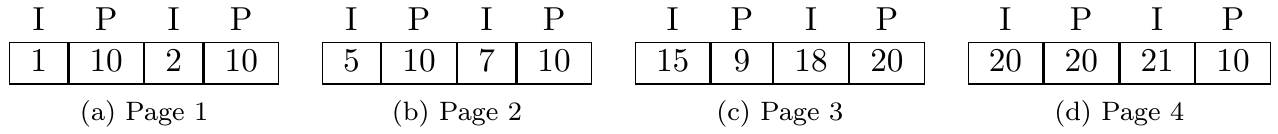
\includegraphics[width=\textwidth]{img/row-store.png}
    \caption{Row store layout.}
    \label{fig:row-column-store-1} 
  \end{subfigure}
  \begin{subfigure}{\textwidth}
    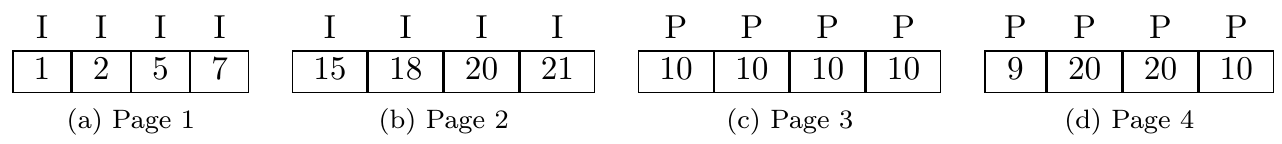
\includegraphics[width=\textwidth]{img/column-store.png}
    \caption{Column store layout.}
    \label{fig:row-column-store-2} 
  \end{subfigure}
  \caption{Row and column oriented layouts for a table with two columns, I and P. In the row-oriented layout (a), records (I and P tuples) are stored next to each other within the pages. In the column-oriented layout (b), values from the I column and P column are stored separately on different pages. Courtesy of \cite{Bjorklund2011-wh}.}
  \label{fig:row-column-store} 
\end{figure}
\section{Column Storage}
\label{sec:Column Storage}


The most common storage format for OLTP systems is row storage, as we briefly mentioned in Section \ref{sec:Definitions}. Row storage enables easy fetching of values from the same tuple, and is suited for updates, inserts, and deletes. However for OLAP workloads, columnar storage has turned out advantageous, mainly because of two reasons: First, aggregations are easier, since calculations are performed on data consecutive in memory. Second, column storage does not fetch more data than is needed for the query.

Our research has identified several systems using columnar storage. These include \monetdb~\cite{Boncz2005-wj, Boncz2002-yj}, \cstore~\cite{Stonebraker2005-qz}, \saph~\cite{Farber2012-vh}, and \mssql~\cite{noauthor_undated-vq, Larson2013-mc}, as well as the \bd~product \tableau~\cite{Kamkolkar2015-iq}.

In a column store, each column in a table is stored separately in a continuous segment (unless data is horizontally partitioned, see Section \ref{sec:Horizontal Partitioning}), as opposed to row stores where attributes from a single row are stored together \cite{Bjorklund2011-wh}. Figure \ref{fig:row-column-store} depicts both row and column oriented layouts for a table with two columns (I and P). The row storage alternates between I and P to store records next to each other on the pages while the column storage keeps I and P values separate. 

The advantages of using column storage are many. The primary one is that no more data is accessed than strictly necessary for a query. In addition to this, columns are inherently more compressible \cite{noauthor_undated-vq}. Compression leads to higher performance due to better cache and memory utilization, and this effect is one of the reasons why \mssql~use column storage. We elaborate on the performance benefits of compression in Chapter \ref{chap:Data Compression}.

Column storage also comes with a more subtle advantage; columns have a \textit{low degree of freedom} compared to row storage \cite{Boncz2005-wj}. When operating on column values, only the local memory offset is required, not the global table layout. This removes some layers of indirection and query processing can be made more efficient. Boncz \ea~claim that this is the main reason why column storage is advantageous.


One of the major disadvantages with column store is that it is not as easily updateable \cite{Bjorklund2011-wh}, especially if the columns are compressed or sorted. This challenge is normally overcome using a separate structure for writes and updates called a \textit{delta store}. Using such structure, the main part of the database is stored column-wise in a static structure optimized for reads while the updates and inserts are accumulated in a smaller and more dynamic structure. We investigate delta stores further in Section \ref{sub:Delta Store}.

Another disadvantage with column storage is tuple materialization costs. Since the result of most DBMS queries should be returned as rows, columns must be stitched back together before returned to the client, an operation that can be expensive.


\subsection{Sorting}
\label{sub:Sorting}
We see that few systems sort the data values before storing them to columns. An exception to this is \cstore, and later \vertica~\cite{Lamb2012-kg, Stonebraker2005-qz}. In these systems, \textit{column projections} can be defined, which is a subset of the columns in a table. Each column projection is sorted based on one column in the subset, which means a column is either sorted by own values or by values from another column in the projection. Projections are specified by the database administrator. A column can have multiple projections, hence multiple sort orders, which results in data duplication. The extra storage needed for multiple column sort orders is justified by the compression that column storage enables.


Sorting values in a column store comes with some advantages. First, single value lookups are easily performed by a binary search (however, this limitation can be overcome by keeping inverted indexes \cite{Lemke2010-is, Schwalb2014-hn}, which we study in Section \ref{sec:Inverted Indexes}) Second, and perhaps most important, is that sorted columns can be compressed aggressively by applying \rle. \rle~is the main reason \cstore~stores sorted data \cite{Stonebraker2005-qz}. We study this type of compression in Section \ref{sec:Run-Length Encoding}.

Column sorting also comes with a performance benefit. Holloway \ea~show how sorted columns perform better due to \rle~\cite{Holloway2008-rr}. \blink~has also reported a performance increase if the columns are sorted prior to testing \cite{Johnson2008-cp}, even if this system does not use \rle.

Except from \cstore~and \vertica, our research has shown little indication that sorting values in columns are common. For instance, \mssql~\cite{Larson2013-mc}, \blink~\cite{Raman2013-em} and \oracle~\cite{Lahiri2015-mz} accept values in the order they appear.

Although most systems do not sort values in the columns and instead accept values as they arrive, many systems have a sorted dictionary when \de~is used. Systems here include \blink~\cite{Johnson2008-cp} and \saph~\cite{Farber2012-vh}. A sorted dictionary has many advantages, like easy lookup for single values, transformation of range predicates to \texttt{IN}-list predicates, and partition pruning. A sorted dictionary structure is better suited for a read-only environment, since updating a sorted dictionary requires some work. We look into \de~in Section \ref{sec:Dictionary Encoding}.

\subsection{Row Stores vs Column Stores}
\label{sub:Row Stores vs Column Stores}
Most research agree that row stores are most suitable for OLTP workloads, and column stores are most suitable for OLAP workloads. Abadi \ea~set out to investigate whether there is a fundamental difference between row and column stores \cite{Abadi2008-dd}. In their research, they used a row store with a vertically partitioned schema to mimic a colum store. They also tried applying indexes to each column such that each column could be accessed independently. Their conclusion was that there \textit{is something fundamental about column stores} that makes them perform so well, and that changes must be made to both storage layer and query executor to obtain the benefits of a column-oriented approach. The main reasons why column storage is better suited for OLAP workloads are:
\begin{itemize}
  \item \textit{Compression}, which we discuss in Chapter \ref{chap:Data Compression}.
  \item \textit{Vectorized execution}, which we discuss in Section \ref{sec:Loop Pipelining and Vectorized Execution}.
  \item \textit{Late materialization}, which we discuss in Section \ref{sec:Late Materialization}.
\end{itemize}

There are situations for OLAP databases where a row store performs better than a column store. A research executed by Holloway \ea~shows that a row store can outperform a column store when processing time is the dominating contraint \cite{Holloway2008-rr}. This is typically the case for low selectivity queries and queries with many predicates. To further improve row storage performance, tuples can be compressed. However, row storage will most likely never beat column stores for OLAP workloads, since bandwidth requirement for processing rows is higher than for columns.

\ffigure{img/chain-reaction.png}{OLTP workloads will affect more than a couple of rows. Index structures must be maintained, and aggregations and materialized views must be updated. In the figure, an update that triggers a chain reaction is depicted. Courtesy of \cite{Plattner2014-fr}.}{fig:chain-reaction}

We have also identified papers that claim OLTP databases also benefit from a columnar storage. The work of Farber \ea~argues that columnar storage is suited for transactional workloads as well, mainly due to the compression \cite{Farber2012-vh}. Also, storing data in columns allows for dropping indexes, which is normally costly to maintain. Last, there are normally a lot more read operations than inserts, updates, and deletes in an OLTP database.

Plattner \ea~claim that most OLTP queries request aggregates instead of single rows \cite{Plattner2014-fr}. In addition, updates to the database normally triggers a chain reaction of updates to indexes and materialized views, as seen in Figure \ref{fig:chain-reaction}. Their conclusion is that column storage is suited for OLTP databases due to efficient aggregation and abscence of indexes. The absence of indexes also makes application development easier, since no performance layer must be specified by the application programmer.

We have earlier in this chapter said that columns are more compressible than rows. However, the work of Holloway \ea~claims that row stores can be compressed just as much if done correctly \cite{Holloway2008-rr}. We believe that even though rows are as compressible as columns, compression of columns is simpler and more practical.

\subsection{Row Identifiers and Tuple Materialization}
\label{sub:Row Identifiers and Tuple Materialization}
A row in a column store is identified by a unique identifier that is common to every value belonging to the same row in a table. Many systems store these IDs implicitly as virtual object IDs (\texttt{void}). A \texttt{void} for an object is calculated using a base ID and the offset from the first value in the column. For instance, the fourth value of a column with base ID 100 has an implicit ID of 103. \texttt{void} type identifiers are used in \monetdb~\cite{Boncz2002-yj}, \cstore~\cite{Stonebraker2005-qz}, \vertica~\cite{Lamb2012-kg}, and \ibm~\cite{Raman2013-em}.

If horizontal partitioning is used, a technique we discuss in the next section, the partition number must also be accounted for in row identification. For instance, \mssql~identifies a row by a combination of row group ID and tuple ID \cite{Larson2013-mc}.

For systems that do not keep columns sorted, stitching together rows is pretty straight forward. All columns selected in a query can be iterated in order and tuples can be materialized before sent back to the client. Needless to say, the operation of stitching together rows comes at a higher cost in a column store than for a row store.

Stitching together columns with different sort orders is a very expensive operation. \cstore~uses join indexes for this operation, which we study in Section \ref{sec:Join Indexes}. \vertica~only allows a query to access columns belonging to the same projection. In other words, a query must use a projection that contains all the columns needed for the query.

\section{Compression}
\label{sec:Compression}
Historically, compression has been thought of a measure for reducing disk usage and memory footprint. However, in our case, compression of data also comes with the benefit of increased performance. A study conducted by Abadi \ea~looked into database compression for in-memory databases, and concluded compression increases performance by a factor of two on average \cite{Abadi2008-dd}.

Among systems we have studied in this research, we have identified several that applies compression for performance reasons. Among these systems are \ibm~\cite{Raman2013-em}, \cstore~\cite{Stonebraker2005-qz}, \vertica~\cite{Lamb2012-kg}, \oracle~\cite{Oracle2015-fs}, and \gorilla~\cite{Pelkonen2015-ko}. In addition to this, our reference products \tableau~and \qlikview~also use compression extensively to achieve good performance \cite{Kamkolkar2015-iq, Qlik2014-vd}. Last, but not least, \exasol, the top performing DBMS in the TPC-H benchmark, applies compression to its data, and uses structures that are designed for rapid retrieval \cite{Exasol2014-xh}.


Compression is beneficial for performance due to:
\begin{itemize}
  \item Cache locality is improved \cite{Exasol2014-xh}. More values from a single column (or record) fit in the cache at the same time.
  \item Memory traffic is reduced. Compression can help turning a program from memory-bound to CPU bound \cite{Willhalm2009-hu}.
  \item Compression can reduce CPU cycles \cite{Stonebraker2005-qz}. First of all, as stated above, it reduces memory latency and improves cache locality, such that more cycles can be used for calculations and not waiting for memory. Besides, compression enables working on multiple values in parallel using SIMD instructions, as we see in Section \ref{sec:SIMD}.
\end{itemize}

Still, even though compression is used to increase database performance, the fact that compression reduces memory usage is also important. Even though DRAM is cheap, it is rarely over-provisioned and unused \cite{Barber2014-ey}. Also, compressed data frees up space for other things, like indexes and result caches. For instance, \oracle~justifies their dual format by using the space freed up by compressing the columns \cite{Lahiri2015-mz, Lamb2012-kg}.

\subsection{Compression Types and Light-Weight Compression}
\label{sub:Compression Types and Light-Weight Compression}
A study performed by Westmann \ea~investigates database compression, and concludes that that the compression must be \textit{light-weight} for maximum performance \cite{Westmann2000-mz}. In other words, the real benefit of compression can only be leveraged if the decompression effort can be minimized \cite{Lemke2010-is}. Light-weight compression has been defined by Holloway \ea~as \bp, \de, \dele, and \rle~\cite{Holloway2008-rr}. Holloway \ea~also conclude that \de~and \rle~are the best compression schemes for column stores. These compression techniques are fast and fine-grained, which is important for performance.

Zukowski \ea~conclude that a compression algorithm should care about super-scalar processors. This implies that the algorithm should be able to pipeline loops, support out-of-order execution, and avoid if-then-else in inner loops \cite{Zukowski2006-oz}. We study these techniques in greater detail in the chapter about hardware utilization (Chapter \ref{chap:Hardware Utilization}). 

A database can use multiple compression schemes. First, most of the light-weight compression techniques can be combined, where the most common combination is \de~and \bp. We study this idea in Section \ref{sec:Dictionary Encoding}. Second, different compression schemes can be used for different columns. In Section \ref{sub:Sorting}, we saw that \cstore~and \vertica~allow for multiple column projections (a subset of the columns), where each projection is sorted based on one of the columns in the subset. This results in each projection having one \textit{self-order} column and several \textit{foreign-order} columns.  \cstore~and \vertica~use the following guidelines when deciding which encoding to use \cite{Stonebraker2005-qz}: 

\begin{itemize}
  \item \textbf{Self-order, few distinct values:} \rle~are used for these columns, where each value is stored once together with how many times the value occurs. We study \rle~in Section \ref{sec:Run-Length Encoding}.
  \item \textbf{Foreign-order, few distinct values:} For each distinct value in a column, a bitmap is stored indicating which rows that contain that value. We study this technique in Section \ref{sec:Compression Using Bitmaps}.
  \item \textbf{Self-order, many distinct values:} \dele~is used. The idea of this scheme is to save the values as a delta from the previous value in the column. We study \dele~in Section \ref{sec:Delta Encoding}.
  \item \textbf{Foreign-order, many distinct values:} Columns are left uncompressed.
\end{itemize}

Later in this chapter, we elaborate on the situations where the various compression schemes are beneficial.

\subsection{Working Directly on Compressed Data}
\label{sub:Working Directly on Compressed Data}

\afigure{img/ram-cache-decompression.png}{I/O-RAM vs RAM-CPU compression. In the left sub-figure, data is decompressed before it is put in the buffer manager (RAM). In the right sub-figure, data is kept compressed in the buffer manager and only decompressed when it is brought into the CPU cache. Courtesy of \cite{Zukowski2006-oz}.}{fig:ram-cache-decompression}{0.6}

In earlier database systems with compression, the data was decompressed when brought up to RAM. In 2006, Zukowski \ea~suggested that data should not be decompressed when moved from disk to RAM, but when brought from RAM to cache \cite{Zukowski2006-oz}, as depicted in Figure \ref{fig:ram-cache-decompression}. \monetx~is a system that decompresses when data is moved from RAM to cache \cite{Johnson2008-cp}.

However, the most performance benefit of compression is seen when the system works on the compressed data directly \cite{Lemke2010-is}. This implies that data should not be decompressed until it is materialized and sent to the user. This principle is backed by the creators of \blink, who says data should never be decompressed before absolutely needed \cite{Barber2012-xt}. \oracle~claims one of the main performance benefits is to work directly on the compressed data \cite{Oracle2015-fs}. Not decompressing data before it is needed relates to a technique known as \textit{late materialization}, a technique we study in Section \ref{sec:Late Materialization}.


\section{Bitpacking}
\label{sec:Bitpacking}

\afigure{img/bitpacking.png}{Bitpacked column values. Values are stored with no more bits than needed to represent the column, which results in values that are not aligned to machine word boundaries. Values may be spread across several machine words and share their machine word(s) with other codewords. Courtesy of \cite{Willhalm2013-ri}.}{fig:bitpacking}{0.8}

\bp~is a trivial form of compression, where values are stored with no more bits than needed. In other words, if a column has a cardinality of 32, only 5 bits are required to represent a value. This way, in a 32-bit architecture, 100 values can be stored using $500$ bits, and not $100*32 = 3200$. \bp~has lower compression than algorithms that allow variable length for values, but values can be randomly accessed in constant time \cite{Raman2008-gi, Willhalm2013-ri}. Also, \bp~enables SIMD processing, which we discuss in Section \ref{sec:SIMD}. \bp~is well suited for high cardinality, uniform distribution of values, where dictionary encoding only provides an unnecessary layer of indirection \cite{Holloway2008-rr}.

As seen in Figure \ref{fig:bitpacking}, bitpacked values will not generally align to word boundaries. For processing, values normally have to be moved to the word boundary, but this cost has been found to be negligible \cite{Holloway2008-rr}. Aligning values can be done in an SIMD like fashion, a technique we study in Section \ref{sec:SIMD}.

In its simplest form, \bp~works directly on the column data, but the compression scheme can be more powerful if combined with other compression types. We see in Section \ref{sec:Dictionary Encoding} that dictionary keys can be bitpacked, and in Section \ref{sec:Delta Encoding} that \dele~benefits from \bp~if the deltas between the values are small. Besides, bitpacked vectors can be used in an inverted index structure \cite{Schwalb2014-hn}, which we study in Section \ref{sec:Inverted Indexes}.

\subsection{Issues with Bitpacking}
\label{sub:Issues with Bitpacking}
\afigure{img/partitioned-bitpack.png}{A normal bitpacked vector (left) and a partitioned bitpacked vector (right). Instead of rebuilding the entire vector on value overflow, the partitioned bitpacked vector has different partitions where each partition is compressed using an increasing number of bits. Courtesy of \cite{Faust2015-ke}.}{fig:partitioned-bitpack}{0.9}
There are two major limitations with \bp~\cite{Faust2015-ke}. The first is that if the bitpacking overflows, the full bitpacked vector must be rebuilt. What this means is that if all values are mapped, such that there are no available values with $n$ bits, a new bit must be introduced, and the entire vector must be rebuilt where each value has $n + 1$ bits. This is depicted in the left part of Figure \ref{fig:partitioned-bitpack}. To counter this effect, Faust \ea~have suggested a partitioned bitpacked vector structure that creates a new partition with $n + 1$ bits on overflow, as seen in the right part of Figure \ref{fig:partitioned-bitpack}. Although this technique improves performance on insert operations, read performance suffers due to the extra overhead of looking up a value.

The second limitation with \bp~is that it does not account very well for data skew. In \bp, each distinct value in a vector contributes to the total number of bits required, completely disregarding the distribution of the values. Often in a database, there are a large number of distinct values, but they are not uniformly distributed. This problem can be solved with the partitioned vectors explained in the previous paragraph, by mapping the values that occur more frequently to the partitions with the fewest bit per value. Other algorithms map outliers to a separate structure, like \pfdelta~\cite{Bjorklund2011-wh}.


\section{Dictionary Encoding}
\label{sec:Dictionary Encoding}
\de, or \term{Dictionary Compression}, is widely used within column store databases. Systems that use \de~include \oracle~\cite{Lahiri2015-mz}, \ibm~\cite{Raman2013-em}, \saph~\cite{Farber2012-vh}, \sapnw~\cite{Lemke2010-is}, \blink~\cite{Johnson2008-cp}, \mssql~\cite{Larson2013-mc}, and more. \qlikview~stores each distinct data point only once \cite{Qlik2011-ef}. \tableau~does not mention anything about \de~in their whitepapers, but an official blog post claims that this compression technique is used \cite{noauthor_undated-us}.

\afigure{img/dictionary-sorted.png}{A sorted dictionary. Each distinct value is stored only once in the dictionary. A key is assigned to each entry in the dictionary, and those keys are stored in the columns instead of the actual values. Courtesy of \cite{Psaroudakis2014-ma}.}{fig:dictionary-sorted}{0.4}

In a dictionary encoded column, each distinct value is stored once in a structure known as \textit{the dictionary}. Keys are assigned to each entry in the dictionary, most commonly integers from zero and up. Columns store these keys and not the actual values, and data is compressed since each unique value is stored exactly once. \de~using a sorted dictionary is illustrated in Figure \ref{fig:dictionary-sorted}. \de~is particularly effective when a column in a column store has only a few distinct values in a large dataset \cite{Faust2015-ke}.


Except from the compression, one of the major advantages of \de, is that many database operations can be performed directly on the encoded values \cite{Faust2015-ke}, which we have seen in Section \ref{sub:Working Directly on Compressed Data} is important to achieve good performance. Integer comparison are less expensive than comparing the actual values, especially for strings. Additionally, range and \texttt{LIKE} predicates can be turned into \texttt{IN}-list operations, since the dictionary can be scanned first to find the relevant integer keys \cite{Barber2012-xt}.

If the columns are partitioned horizontally, which we have discussed in Section \ref{sec:Horizontal Partitioning}, it is common that each partition has a separate dictionary. This is the case for most database systems, like \oracle~\cite{Lahiri2015-mz}, \blink~\cite{Barber2012-xt}, and \mssql~\cite{Larson2013-mc}. When a dictionary is stored per partition, it can be used for quick data pruning; if a value is not present in the dictionary, the partition can be skipped. \blink~and \monetx~use this technique \cite{Barber2012-xt, Boncz2005-wj}. 

When implementing \de, special considerations should be taken. First, if the dictionary turns out bigger than the values it is replacing, \de~should not be used \cite{Holloway2008-rr}. Secondly, \de~performs best if the dictionary fits inside the L2 cache of a processor.

Like \bp, \de~does not handle data skew very well, since each unique value needs an entry in the dictionary no matter how frequent that value appears in a column. Besides, for high cardinality columns, the compression is less efficient.

\subsection{Sorted Dictionaries}
\label{sub:Sorted Dictionaries}
Dictionaries can be either sorted or unsorted. Using a sorted dictionary enables easier value lookup using a binary search. However, more important for us, is that using a sorted dictionary can turn range scans into simple integer comparisons \cite{Faust2015-ke}. For instance, if we want to find all sales in 2010, we only need to look up the integer codes for January 1st, 2010 and January 1st, 2011 and find all integers within this range. Since integer comparisons are fast and effective, this technique will usually improve performance. 

Most database systems today use sorted dictionaries. \saph~is an example of such system \cite{Farber2012-vh}.

However, as briefly mentioned in Section \ref{sub:Sorting}, keeping a dictionary sorted implies a higher overhead on database inserts, updates and deletes. We see in Section \ref{sub:Delta Store} that some systems divide their data into two stores: A read-optimized store, and a delta store (for updates and inserts). With this division, it is common to use a sorted dictionary for the read-optimized store and an unsorted dictionary for the delta store \cite{Plattner2014-fr}.

\subsection{Dictionary Encoding and Bitpacking}
\label{sub:Dictionary Encoding and Bitpacking}
\de~is commonly used in conjunction with \bp. With this combination, the dictionary keys in the columns are stored with no more bits than necessary. Since dictionary keys normally are integers from zero to the number of entries, bitpacking enables high compression rates, especially for low-cardinality columns.

Systems using \de~and \bp~include \ibm~\cite{Raman2013-em}, \blink~\cite{Barber2012-xt}, \sapnw~\cite{Willhalm2009-hu}, and \saph~\cite{Psaroudakis2014-ma}. \qlikview~has also reported to compress data with only the number of bits required \cite{Qlik2014-vd}. \mssql~does not apply \bp~on dictionary keys in columns, and instead store them as 32-bit integers \cite{Larson2013-mc}.

The same advantages and disadvantages of \bp~apply to \de~with bitpacked columns. For instance, values can be looked up in constant time and queries can be processed in an SIMD-like fashion. However, insertions to the dictionary might lead to an overflow, which requires the entire column to be rebuilt.

\section{Background Information on Modern CPUs and Compilers}
\label{sec:Background Information on Modern CPUs and Compilers}
Modern processors are capable of performing an enormous amount of calculations per second, but that depends on the amount of available and independent work. The instructions-per-second (IPC) difference between minimal and maximal CPU utilization can easily be one order of magnitude \cite{Boncz2005-wj}. Hence, database software must be implemented such that it fully exploits the processing power made available by the CPU.

\subsection{Pipelining, Superscalar Processing, and Independent Instructions}
\label{sub:Pipelining, Superscalar Processing, and Independent Instructions}
\afigure{img/superscalar.png}{A simple superscalar pipeline. Multiple execution units allow for processing multiple instructions in parallel. Courtesy of \cite{Wikipedia_contributors2015-kp}.}{fig:superscalar}{0.6} 

Modern processors improve clock rate and IPC by using a technique known as \textit{pipelining} \cite{Boncz2005-wj}. By dividing an instruction execution into multiple steps, there is less work per stage, and the CPU frequency can be increased. Figure \ref{fig:superscalar} depicts an example pipeline with five stages. However, pipelining also introduce two dangers; \textit{instruction dependencies} and \textit{branch misprediction}.

In a pipeline, \textit{dependencies between instructions} impose a problem. If an instruction is dependent on another, it must wait for the other instruction to complete before it enters the pipeline. Dependent instructions can severely hurt performance, especially if the pipeline is long.

Conditional branches are also affected by dependencies between instructions. When executing a conditional branch instruction, the decision whether to take a branch is usually dependent on the result of a preceding instruction \cite{Boncz2005-wj}. To avoid stalling the pipeline when waiting for the expression to evaluate, modern CPUs use a technique known as branch prediction where the processor immaturely starts executing the branch that is most likely to be taken. The performance penalty occurs if a branch is \textit{mispredicted}, where the instructions in the pipeline must be invalidated (pipeline flushing).

Another way that performance is increased in a processor is by having muliple execution units. We refer to such processors as \textit{superscalar}. As seen in Figure \ref{fig:superscalar}, a superscalar processor can have multiple instructions in the same stage of the pipeline, which allows IPC (instructions per cycle) $> 1$. However, for this functionality to be fully utilized, independent work is required.

\begin{figure}
  \centering
  \begin{subfigure}{0.45\textwidth}
    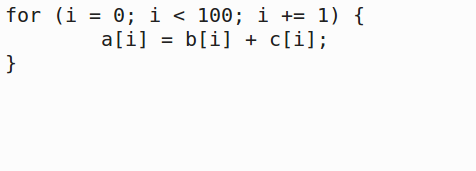
\includegraphics[width=\textwidth]{img/loop-unrolling-1.png}
    \caption{Original loop}
    \label{fig:loop-unrolling-1} 
  \end{subfigure}
  \begin{subfigure}{0.45\textwidth}
    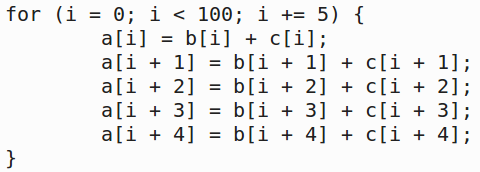
\includegraphics[width=\textwidth]{img/loop-unrolling-2.png}
    \caption{Unrolled loop}
    \label{fig:loop-unrolling-2} 
  \end{subfigure}
  \caption{By unrolling loops, instructions are made independent and the number of branches is reduced.}
  \label{fig:loop-unrolling} 
\end{figure}
Hence, to reach maximum performance for a pipelined, superscalar processor, we must find independent work. Since most programming languages do not let the programmer specify which instructions are independent of each other, compiler optimizations play a critical role in CPU utilization \cite{Boncz2005-wj}. The most widely used technique used by the compilers to address this challenge is \textit{loop unrolling}, which is used to reduce the number of branches and increase independence between instructions \cite{Wikipedia_contributors2015-zc}. As seen in Figure \ref{fig:loop-unrolling}, loop unrolling reduces the number of iterations in a loop (reduction of branches) and replaces it with multiple instances of the same instruction. If the instructions are independent, they can be processed in parallel.

\subsection{CPU Caches}
\label{sub:CPU Caches}
Since transfering data from main memory to CPU can take around $~200$ cycles, modern CPUs utilize multiple layers of on- and off-chip caches to reduce this latency. Efficient usage of caches is paramount for CPU throughput, since roughly 30\% of all instructions in a program are memory loads or stores \cite{Boncz2005-wj}. We know that IPC for DBMSes is strongly impaired by cache misses, and cache utilization is an important topic for in-memory databases \cite{Exasol2014-xh}.

The best way to tackle this challenge is to design algorithms and data structures that are \textit{cache aware} \cite{Farber2012-vh}. Designing such programs is out of the scope of this report, but it briefly boils down to two things:
\begin{itemize}
  \item \textit{Coordinate temporal and spatial locality}. Data processed together should be stored at consecutive memory addresses. Code locality is also important \cite{Neumann2011-uq}.
  \item \textit{Avoid false sharing of cache lines}. Multiple cores in a processor should not write to data belonging to the same cache entry at the same time to avoid unecessary invalidations.
\end{itemize}
\textit{Compression}, which we described in Chapter \ref{chap:Data Compression}, and \textit{vectorized execution}, which we discuss in Section \ref{sec:Loop Pipelining and Vectorized Execution}, are two techniques used to improve cache performance \cite{Larson2013-mc, Lemke2010-is}.

\textit{Prefetching} is another method used to increase cache utilization. Prefetching proactively loads data into caches such that the data is available when an instruction needs it.

\subsection{Call Stack and Subroutine Invocations}
\label{sub:Call Stack and Subroutine Invocations}
\afigure{img/call-stack.png}{A call stack for a program in execution. Each stack frame contains input parameters, function return address, and local variables for a subroutine invocation. Courtesy of \cite{Wikipedia_contributors2015-od}.}{fig:call-stack}{0.5}

A \textit{call stack} is commonly used in a computer program to store information and state about active subroutines \cite{Wikipedia_contributors2015-od}. Each time a subroutine is called, a \textit{stack frame} is added to the call stack that stores the input arguments, return address, and variables local to the subroutine. See Figure \ref{fig:call-stack}. The call stack can be implemented in both hardware and software, and the implementation varies between different systems. This stack-based technique implies that calling a subroutine comes at a cost; registers must be stored on the stack, and a new stack frame must be added.

Trading off time with space is usually done to address the above challenge; adding more code to improve program efficiency. \textit{Function inlining} is a technique used by compilers where the subroutine code is copied into the caller's body. This way, no new stack frame is created for the subroutine, avoiding the overhead associated with a function invocation.

\textit{Macro expansion} is another form of code generation. Macros are normally specified by the application programmer, and can be used for programmer-controlled inlining of functions or constant values. Macros can also be used to generate multiple versions of function or class definitions (templating), a technique commonly used to let a single implementation support different data types.

\section{Branch Avoidance}
\label{sec:Branch Avoidance}
\ffigure{img/branch-selectivity.png}{Predicate evaluation performance for queries with different query selectivities. A \textit{branch version} and a \textit{predicated version} are tested. For the AthlonMP processor, the branch version are 2-3 times slower on queries with 40\%-60\% selectivity, while the Itanium2 processor has constant processing time. The predicated version offers constant processing time for both processors. Courtesy of \cite{Boncz2005-wj}.}{fig:branch-selectivity}

We saw in the previous section that branches should be avoided due to the penalties of branch misprediction. Besides, branches also cause dependencies between instructions. 

The consequences of inaccurate branch prediction are studied by Neumann \ea~\cite{Neumann2011-uq}. In this research, the performance of queries with various selectivities was tested. As we can see in Figure \ref{fig:branch-selectivity}, queries with 40\%-60\% selectivity executed on an AthlonMP processor are roughly 2-3 times slower than queries with selectivities close to 0\% or 100\%. Hence, selectivity can severely affect the query performance. The Itanium2 processor does not have the same characteristic, as the Itanium architecture allows for both \textit{not taken} and \textit{taken} branches to be executed simultaneously.

Neumann \ea~also developed a branchless version (predicated version) to evaluate predicates in the queries. The branchless variant is denoted as \texttt{predicated version} in Figure \ref{fig:branch-selectivity}. For both AthlonMP and Itanium2 processors, this implementation offers constant performance for all selectivities, but is, in general, more expensive.

Branch avoidance is also important in other parts of the system, for instance when decompressing. Zukowski \ea~present a decompression algorithm that is free for \textit{if-then-else} statements \cite{Zukowski2006-oz}. By running the algorithm in two tight loops instead of one, branch misprediction is reduced, and the loops can be pipelined by a compiler.

Branches can also be avoided by compiling queries to machine code \cite{Lamb2012-kg}. We will elaborate on this technique in Section \ref{sub:Compiling Queries to Machine Code}.

\subsection{Short-Circuiting}
\label{sub:Short-Circuiting}
\begin{figure}
  \centering
  \begin{subfigure}{0.45\textwidth}
    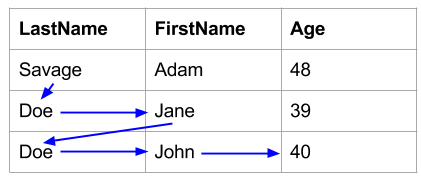
\includegraphics[width=\textwidth]{img/short-circuiting-1.png}
    \caption{Short-circuiting}
    \label{fig:short-circuiting-1} 
  \end{subfigure}
  \begin{subfigure}{0.45\textwidth}
    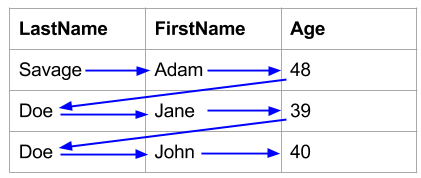
\includegraphics[width=\textwidth]{img/short-circuiting-2.png}
    \caption{No short-circuiting}
    \label{fig:short-circuiting-2} 
  \end{subfigure}
  \caption{Predicate evaluation for query \texttt{WHERE LastName='Doe' AND FirstName='John' AND Age>21}. (a) skips evaluating rest of the predicates if one predicate is false, while (b) evaluates all predicates regardless of previous results.}
  \label{fig:short-circuiting} 
\end{figure}
\textit{Short-circuiting} is referred to a special case of Boolean operator evaluation in which the next argument is not evaluated if the current argument is sufficient to determine the value of the expression \cite{Wikipedia_contributors2015-rk}. Figure \ref{fig:short-circuiting} illustrates the difference between short-circuit and non-short-circuit predicate evaluation. In short-circuiting, the scan proceeds to the next tuple as soon as one predicate is false, as opposed to the verision without short-circuiting that evaluates all predicates regardless of previous results.

Since short-circuit boolean operators are control structures and not simple arithmetic operators, there is a chance of branch misprediction. That is why \blink~does not short-circuit between tuples \cite{Raman2008-gi, Johnson2008-cp}. If a block is selected for scanning, all fields in the records are checked. According to Raman \ea, short-circuiting only improves performance on low selectivity queries \cite{Raman2008-gi}.

\subsection{Cache Awareness}
\label{sub:Cache Awareness}
We saw in Section \ref{sub:CPU Caches} that efficient utilization of caches is important for database performance, so data structures and algorithms should be designed such that they are cache-aware. Our research has identified several systems that are designed to be cache-aware, including \monetdb~\cite{Boncz2002-yj}, \mssql~\cite{Lahiri2015-mz}, and \ibm~\cite{Raman2013-em}. The developers of \exasol, the top performing database system in the TPC-H benchmark, claim that high level of data locality is one of the key factors to performance.

\subsection{Macro Expansions}
\label{sub:Macro Expansions}
\afigure{img/macro-expansion.png}{Macro expansions in \monetdb. For different algorithms and data types, the \texttt{select} operator has a total of 173 implementations. Courtesy of \cite{Boncz2002-yj}.}{fig:macro-expansion}{0.6}

\monetdb~uses macro expansion to reduce layers of indirection and to optimize query execution performance \cite{Boncz2002-yj}. Since operators normally are type-generic, \monetdb~has for each algorithm multiple implementations that are specific to a certain type. The implementations are generated automatically using macros, which is why they are called \textit{macro expansions}. Figure \ref{fig:macro-expansion} shows how the \texttt{select} operator is expanded into 173 implementations, depending on which algorithm and data types are queried.

The vector data structure in \ibm~is implemented using C++ templates to support multiple data types.



\section{Other Database Topics}
\label{sec:Other Database Topics}

\subsection{Bitmap Indexes}
\label{sub:Bitmap Indexes}

\ffigure{img/bitmap-query.png}{Executing a query using bitmap indexes. Queries are efficiently processed using bitwise operations like \texttt{AND} and \texttt{OR}. Courtesy of \cite{noauthor_undated-hp}.}{fig:bitmap-query}

A \biti~is a particular structure where a bitmap represents each distinct value in a column, and all rows containing that value is set to 1. As we have seen in Section \ref{sec:Compression Using Bitmaps}, replacing columns with bitmaps can reduce the storage requirements for a column. However, the bitmaps can also aid predicate evaluation as the form of a \biti. A \biti~is most efficient on queries that contain multiple \texttt{WHERE} clauses since many candidate rows can be excluded using bitwise \texttt{AND} and \texttt{OR} operations, as seen in Figure \ref{fig:bitmap-query} \cite{noauthor_undated-hp}. Since bitmap indexes combine so easily, composite indexes are extraneous. 

One of our reference products, \qlikview, reports that it uses binary indexes for each field \cite{Qlik2011-ef}, which we believe are the same as bitmap indexes. Some database management systems also support bitmap indexes, including \oracle~\cite{noauthor_undated-hp} and \ibm~\cite{Raman2013-em}.

In general, low-cardinality columns, which is columns with few distinct values, are better suited for bitmap indexes than high-cardinality columns \cite{noauthor_undated-hp}. The reason for this is because a bitmap must be created and maintained for each unique value in the column. Besides, since these indexes are hard to maintain, they are not suited for inserts, updates, and deletes. When deciding whether to add a \biti~to a column, \oracle~recommends at least 100 rows per distinct value. 

Bitmap indexes may also be used as join indexes, and is much more efficient in storage than storing pre-joined materialized views \cite{noauthor_undated-hp}. We study join indexes in Section \ref{sec:Join Indexes}.

\subsection{Joining}
\label{sub:Joining}
Joining is a common database operation that combines records from two or more tables. In our research, we have studied several DBMSes, and seen how their join algorithms work. As we saw in Section \ref{sub:Business Discovery, Queries, and SQL}, joining is also needed for a \bd~application such that interaction with one table can affect the selection, filters, or aggregations in other tables.

For joining two tables, three main methods exist \cite{Bratbergsengen2015-ed}: 
\begin{itemize}
  \item \textit{Partition-based approach}, where records of both tables are split into groups based on the hash value of the keys. This technique is most effective on data volumes that are too large to fit in main memory.
  \item \textit{Sort-merge approach}, where both tables are sorted and then merge results by concatenating records with equal key values. This approach is most effective when one or both operands are sorted in advance.
  \item \textit{Nested loop approach}, which compares all rows in both tables.
\end{itemize}

We find the \textit{nested loop} approach to be the most popular joining algorithm for in-memory and parallel databases \cite{Boncz2002-yj}. The rest of Section \ref{sec:Joining} will therefore only discuss this method.

\subsection{Nested Loop Algorithms}
\label{sub:Nested Loop Algorithms}

% Basic nested join functionality
In its simplest form, the \textit{nested loop} method compares the join key in all rows directly using a double loop. This simple algorithm has a runtime of $O(n*m)$ where $n$ and $m$ is the size of tables A and B respectively. However, to improve performance in a \textit{nested loop} algorithm, hashmaps are commonly used. Usually, the join is performed by hashing the smaller (inner) relation first, then probe the hashmap by scanning the larger (outer) relation. 

In a star or snowflake schema, dimension tables are usually considered as the inner relations \cite{Barber2012-xt, Raman2013-em}. In other words, the keys of these tables will be used to create the hashmaps in the join. In the second phase of the algorithm, the fact table will probe the generated hashmaps to complete the join. 

\ffigure{img/nested-loop.png}{An example nested loop join structure. Records are first tested against a Bloom filter. If found in the filter, the join key is searched in the join structure. Records are first hashed, and then each entry in the hash table is the root of a binary tree. Courtesy of \cite{Bratbergsengen2015-ed}.}{fig:nested-loop}

Kjell Bratbergsengen shows how a combination of hash tables, bloom filters, and binary trees can be used in a \textit{nested join} algorithm. In the probe phase, keys are first checked towards a Bloom filter (Section \ref{sub:Bloom Filter}). Bloom filters never return false negatives and is an efficient way of reducing the numbers of keys entering the join. If the key is found in the Bloom filter lookup, it is hashed and checked up against a hybrid hashmap/binary-tree structure. In this structure, each entry in the hashmap is the root node of a binary tree which are used to efficiently look up values. The join algorithm is illustrated in Figure \ref{fig:nested-loop}.

% Modifications
In the nested loop approach, one of the operands might be partitioned \cite{Bratbergsengen2015-ed}. For example, a join might be partitioned by only hashing a subset of the inner relation at a time. The entire join algorithm will then include several probe passes over the outer relation, one for each subset. Historically, this technique has been applied to ensure the whole hash structure fits in RAM. We conclude that a similar concept can be applied to CPU caches and that the join algorithm might benefit from partitioning the inner relation such that each subset fits in the CPU cache.

We see that several DBMSes in this research use a \textit{nested loop} join variant with Bloom filters, including \oracle~\cite{Lahiri2015-mz}, \ibm~\cite{Raman2013-em} and \blink~\cite{Raman2008-gi}. Barber \ea~explains how Bloom filters are effective in eliminating non-matching join outers before they enter the join \cite{Barber2014-ey}.

Our research has shown that one of the key design goals for efficient joining using the \textit{nested loop} approach with hashmaps, is to keep the hash tables collision free \cite{Raman2008-gi, Raman2013-em}. One way to ensure this is to use the dictionary keys in \de~as a perfect hashing function. If a table is joined on several keys, a minimal perfect hash can be calculated.

Regarding implementation, it is important that the algorithm and the hash table are \textit{cache-aware}. One way to improve cache performance in a \textit{nested loop} join, is to use linear probing instead of open-chain addressing for the hashmap \cite{Raman2008-gi}. Open-chain addressing should only be used for overflow buckets.

Joining should be done in parallel for ultimate performance. For instance, the hash tables can be built using multiple threads \cite{Barber2014-ey}. We see that some \textit{nested loop} based algorithms partition the input to improve cache performance. However, this decision might as well be a parallelization decision \cite{Neumann2011-uq}. A system studied in our research that employs high-performance parallel joining is \ibm~\cite{Raman2013-em}.

\subsection{Database Statistics}
\label{sub:Database Statistics}
\term{Database Statistics} are commonly used by a query optimizer to make better decisions about creating efficient execution plans. These statistics may the include number of records, selectivity, column cardinality, value distribution, and more. In our case, \term{Database Statistics} can be used to prune horizontal partions based on the column minimum and maximum values. This technique exploits clustering in the columns, especially when the columns are sorted, or partially sorted, like timestamps. \oracle~\cite{Lahiri2015-mz}, \ibm~\cite{Raman2013-em}, \vertica~\cite{Lamb2012-kg}, \monetx~\cite{Boncz2005-wj}, \mssql~\cite{Larson2013-mc}, and \exasol~\cite{Exasol2014-xh} store partition metadata for quick data pruning.

Most database systems keep the statistics stored together with the table. However, other schemes exist. \ibm~uses a synopsis table to keep track of all column pages (partitions), including minimum and maximum values. This way, irrelevant pages can easily be skipped \cite{Raman2013-em}.

We have previously discussed how a partition dictionary can be checked for a key's existence before scanning an entire block. If a key is not present in the dictionary, the partition can be skipped. We consider this technique as a part of utilizing \term{Database Statistics} to improve performance.

It can sometimes be useful to know a column's value distribution. For instance, the frequency partitioning in \blink~and \ibm~uses the columns' value distributions when determining how to partition the data \cite{Raman2008-gi, Raman2013-em}. The query optimizer in \mssql~also uses the value distributions when creating execution plans \cite{Larson2013-mc}. Value distributions are usually determined by creating histograms, and to make these histograms, random sampling can be used. In \mssql, two techniques are used: One is truly random, where values are picked across the whole column, and one is a grouped version, where a random sample range is picked.

\section{Business Discovery}
\label{sec:Business Discovery}
To overcome the challenges with traditional \bi~systems, a new type of products have emerged. We call these for \bd~products, a notion that was introduced by \textit{Qlik}~\cite{Qlik2014-vd}. \bd~products normally build on in-memory technologies and are fast, elegant, and end user intuitive solutions to analyse business data. Examples of such products are \powerpivot, \tableau, and \qlikview. We have only studied \qlikview~and \tableau~in this thesis.

\ffigure{img/qlik-hierarchy.png}{Comparison of a traditional reporting application and \qlikview. Traditional \bi~applications normally have predefined drill-down paths. \qlikview~allows the user decide where to start and end. Courtesy of \cite{Qlik2014-vd}.}{fig:qlik-hierarchy}

\bd~products allow users to follow their "information scent" or "train of thought" when navigating through the data \cite{Kamkolkar2015-iq, Qlik2014-vd}. As seen in Figure \ref{fig:qlik-hierarchy}, there are no prespecified drill-down patterns, and users decide where to start and end. In these applicaitons, grouping, joining, and calculations are performed on-the-fly. High-performance, in-memory technologies are used to enable such functionality. 

In the next sections, we explain how a typical \bd~application works by using \qlikview~primarily as an example. \tableau~and \powerpivot~work similarly.

\subsection{Data Import}
\label{sub:Data Import}

\ffigure{img/qlikview-script.png}{The \textit{Edit Script} dialog in \qlikview. The import script specifies data sources and defines tables and associations for the data that should be analyzed. Courtesy of \cite{QlikTech_International_AB2011-ov}.}{fig:qlikview-script} 

Data is loaded into a \qlikview~document using a data import script that connects the application with data sources like databases or files. The script uses an SQL-like syntax that lets the user specify names of fields and tables that are used in the data analysis. Also, database connection parameters or file paths are stored. Figure \ref{fig:qlikview-script} shows the dialog used in \qlikview~to configure a data import script.

When the data import script is run, data is fetched from the sources and put into the \qlikview~in-memory engine such that data can be queried efficiently. In \qlikview, no queries are executed directly on the underlying data sources. \tableau, however, allows this. In addition to the built-in in-memory engine, the application can be connected directly to live database servers such that companies can utilize investments in high-performance databases \cite{Kamkolkar2015-iq}.


\afigure{img/qlikview-association.png}{Four tables: Countries, customers, transactions, and memberships. The fields \textit{Country} and \textit{CustomerID} associate the tables. Courtesy of \cite{QlikTech_International_AB2011-ov}.}{fig:qlikview-association}{0.6}

The data import script will regularly include more than one table. Multiple tables are \textit{associated} if they have fields with the same name, as seen in Figure \ref{fig:qlikview-association}. Internally, there can be only one data connector between a pair of tables, so if multiple tables refer to a single table, a mechanism (either \textit{synthetic keys} or \textit{loose coupling}) must be applied to logically duplicate the table. This restriction ensures that there exists no more than one possible join path between any pairs of tables \cite{noauthor_undated-js}.

In the data import step, data might be preprocessed and transformed. First, data can be aggregated, for instance by summarizing or grouping, before being loaded into \qlikview. Second, data might be filtered. Both these techniques reduce data volumes. Lastly, data can be denormalized in the import script, i.e. pre-joining tables before import. Denormalizing can be done to lower the number of tables in the data extract and, by doing so, reduce application complexity. We discuss the performance impact of pre-aggregating and denormalization in Section \ref{sec:Application Design} and Section \ref{sec:Denormalization} respectively.

\subsection{User Interface}
\label{sub:User Interface}
\ffigure{img/qlik-panel.png}{\qlikview~dashboard with various GUI elements, like lists and charts. Selections are green, matched data is white, and unrelated data is gray. Courtesy of \cite{Qlik2014-vd}.}{fig:qlik-panel}
Users interact with the \bd~application through a reporting dashboard, as seen in Figure~\ref{fig:qlik-panel}. Requirements for such panel are typically \cite{Qlik2014-vd}:
\begin{itemize}
  \item Clicking field values in list boxes.
  \item Lassoing data in charts, graphs, and maps.
  \item Manipulating sliders.
  \item Choosing dates in calendars.
  \item Cycling through different chart types.
\end{itemize}

Users navigate through the data by making selections in the user interface. When a selection is made, the item is made green, as seen in Figure \ref{fig:qlik-panel}. The current selection is also known as the \term{application state}. Upon selection, the rest of the elements in the panel are updated based on the new application state; aggregations are recalculated, and graphs and lists are updated. \qlikview~colors matched elements white and unmatched elements gray.

Both \qlikview~and \tableau~publish the reporting dashboards through a server \cite{Kamkolkar2015-iq, Qlik2011-ef}. This way, the dashboards are accessible for multiple users at the same time, and can be accessed from different devices, including desktop computers, tablets, and mobile phones.

\subsection{Security Settings}
\label{sub:Security Settings}
In \qlikview, document-level authorization is the main form of access control \cite{Qlik2011-hj}. Here, documents (data extracts and reporting panels) may be restricted and only made available to certain users or user groups. In addition to document-level authorization, applications may also define a dynamic filter that is applied to the data. Using this dynamic filter approach, several user groups can use the same document, only with different restrictions on the data.

\tableau~supports both data-level and user-level security \cite{Kamkolkar2015-iq}. Data can be filtered per user as long as the filter matches a \texttt{WHERE}-clause. Like \qlikview, \tableau~can restrict the access to reports and views to certain users or user groups.

\subsection{Business Discovery, Queries, and SQL}
\label{sub:Business Discovery, Queries, and SQL}
We see that \bd~products interact with the data using selections and filters in a reporting panel. This technique is different from database systems designed for OLAP workloads, which normally use a \textit{query-based} interface, usually SQL. Since we study several DBMSes in this report, it is important to know how \bd~products relate to traditional database queries and SQL.

Queries, or requests, in a \bd~application have certain characteristics. First of all, they cannot be anticipated, more specifically, they are \textit{ad-hoc}. Secondly, there is a limit to the number of returned rows. Users are interested in queries that can be analyzed quickly, so we do not expect a \bd~application to return thousands of rows as a result from a single table \cite{Ferrari2012-hm}. Also, the user interface has limitations in how much data that can be displayed at the same time. 

Even though \bd~applications do not support traditional queries, they still need most of the functionality provided by SQL. Below, we enumerate core SQL functionality and explain why it is necessary in order to create a \bd~application.

\paragraph{Listing of rows}
\bd~applications require rows in a table to be listed in the user interface. Although this seems like a trivial requirement, there are storage formats (Column Storage, Section \ref{sec:Column Storage}) where listing and "stitching together" tuples are non-trivial. 

\paragraph{Filtering}
We need data filtering in a \bd~application for several reasons. First and foremost, application state might be specified in terms of a predicate. For instance, the user might want to display transactions between two dates. Secondly, to support security, some data might need to be filtered before sent to the application.

\paragraph{Joining}
We see that \bd~applications work on several associated tables at a time. Hence, joins are required to connect the tables such that one table can be filtered based on a selection in another table. However, we can limit our join functionality to equijoins over foreign keys. Join functionality is not needed if the imported data is denormalized and put into one single table.

\paragraph{Grouping and aggregation}
\label{par:Grouping and aggregation}
As mentioned earlier, we expect \bd~applications to include summaries of data which is the reason grouping and aggregation must be supported. We may limit the grouping keys to foreign key attributes.

\paragraph{Sorting}
\label{par:Sorting}
Sorting is required in a \bd~application because there will be GUI elements that keep their data sorted. Although this can be solved in the client, it is better to do this during query processing. Besides, we need sorting if we want to show the top of a selection, for instance, the top ten grossing products.

\section{Testing}
\label{sec:Testing}
The TPC-H benchmark is commonly used to test analytical workloads. The benchmark is made for decision support workloads and consists of a suite of business oriented ad-hoc queries \cite{Transaction_Processing_Performance_Council_TPC2014-ux}. The benchmark has 22 complex read-only queries, which are both memory and CPU bound \cite{Boncz2005-wj}, and two update queries for data refresh. The TPC-H specification says the benchmark illustrates a decision support system that:
\begin{itemize}
  \item Examine large volumes of data.
  \item Execute queries with a high degree of complexity.
  \item Give answers to critical business questions.
\end{itemize}

\afigure{img/tpc-h.png}{The TPC-H schema. Courtesy of \cite{Transaction_Processing_Performance_Council_TPC2014-ux}.}{fig:tpc-h}{0.8}
The schema for the TPC-H benchmark consists of eight separate tables, as seen in Figure \ref{fig:tpc-h}. The table columns have a variety of different data types, including integers, floating points, variable and fixed width strings, identifiers, and booleans. 

\afigure{img/tpc-h-population.png}{TPC-H database size and cardinalities. Courtesy of \cite{Transaction_Processing_Performance_Council_TPC2014-ux}.}{fig:tpc-h-population}{0.8}
Figure \ref{fig:tpc-h-population} shows the minimum population for the TPC-H benchmark, which is a database of 10,000 suppliers and roughly 6 million line-items (items per order). The minimum population corresponds to roughly 1 GB. To test larger data sizes, a scaling factor is commonly applied to increase the size of the dataset. According to the specification, data in the tables should be uniformly distributed.

The TPC-H benchmark tests uniformly distributed data, but, in reality, it is quite common that data is skewed. For instance, a retailer might expect that 99\% of the sales are performed on weekdays, and around 40\% of the total sales for a year is done around Christmas \cite{Raman2008-gi}. Tests on data with non-uniform distributions should be performed to see how the algorithms and data structures in the database handle outliers. Data skew can be modelled with a \term{Zipfian} distribution \cite{Holloway2008-rr}. 


\section{Model-driven Development}
\label{sec:Model-driven Development}
Model-driven development is defined as *. Developers have always wanted to raise programming abstraction levels \cite{Atkinson2003-wr}.

\todo{Insert from Atkinson 2003 here}

\mendix, one of the market players in \mdd, uses a JavaScript blabla.

We investigate \gap in the following chapter.

\subsection{Model levels}
\label{sub:Model levels}
\afigure{img/linguistic-metamodeling.png}{Linguistic metamodeling view. Courtesy of \cite{Atkinson2003-wr}}{fig:linguistic-metamodeling}{0.8}
According to Leppänen M, a model is a thing that is used to help the understanding of some other things \cite{Leppanen2006-ay}. In his framework, he describe three different levels of models: The instance model, the type model, and the meta model. A meta model is something used to help the understanding and communication analysis and design of type models. A model on a higher level describes/ prescirbes models on teh next lower level.

% Ønsker å bruke disse nivåene, kanskje med eksempler fra Bergheim.
They also correspond to the information system layer, information system development layer, the method engineering layer, and research work layer.

Although there are many ways to define these levels, we list the levels defined by Bergheim et al.
\begin{itemize}
    \item Operational level - Changes of state in an application
    \item Next meta level - Descriptions of a specific application
    \item B-level - how to make programming tool, like the java programming language itself
    \item Higest level is to make intances on feth B level, how to make different formalisms.
\end{itemize}

\section{Delphi Programming Language}
\label{sec:Delphi Programming Language}
Since the system we will study in this thesis, the \gap, we need to study some background theory of how this language works. \delphi~is both a programming language and an integrated development environment \cite{Wikipedia_contributors2016-jk}, but we will only consider the programming language in this section. The language is an \name{Object Pascal} dialect and compiles into native code for several platforms, including \name{OSX} 32-bit architecture and \name{Windows} 32- and 64-bit architectures. It has a more efficient compiler than most languages. Delphi is classified as a strongly typed high-level language. Delphi supports object oriented design with polymorphism and interfaces.

Delphi support strings with reference counting \cite{Wikipedia_contributors2016-jk}, and the memory for such is managed without programmer intervention. It supports unicode strings.

In 2009, generics and full unicode support was introduced.

A program in \delphi~is composed of different units, with two mandatory parts: The interface, much like a header in C, that declares constants, types, variables, and functions that are available from the outside, and the implementation, that contains the actual code \cite{noauthor_undated-pl}. Types, variables, etc. that are declared in the implentation part only are inaccesible outside the unit. In addition, each unit might specify an initialization and finalization code chunk to run on unit load and unit unload respectively. One unit may depend on other units by specifying the dependencies in the \texttt{uses}. Hence, the dependency graph is automatically created and no makefiles are needed. Cricular dependencies cause compilation error, and are not resolved automatically \cite{noauthor_undated-sp}.

It supports preprocessing directives, but not macros.

\delphi~has operators for referencing and dereferencing values, and supports basic pointer arithmetic \cite{noauthor_undated-cn}.

\subsection{Delphi Types}
\label{sub:Delphi Types}

Simple types can be divided into two categories: Ordinal and real \cite{noauthor_undated-st}. Integer types is one of the ordinal value types, and have both platform-dependend and platform-independent implementations. Platform-dependent is always encouraged due to performance benefits.

\subsubsection{String Types}
\label{ssub:String Types}
\afigure{img/delphi-strings.png}{Strings in \delphi}{fig:delphi-strings}{0.8}
There are two major character implementations, \cn{AnsiChar} and \cn{WideChar}, with 1 or 2 bytes each respectively. The latter is default.

There is support for both single and double precision floating point numbers.

There are both Ansi and Unicode strings, where the default is Unicode \cite{noauthor_undated-cp}. There is support for both UTF-8 and UTF-16 encodings. The latter is default. Both strings are dynamically allocated, and is limited by the available memory. They are allocated on the heap. A string variable is a pointer with reference counting, length, data length and code page. The compiler tries to exploit the nature of the reference counting, and it has copy-on-write semantics if one reference changes the string. Unicode strings defaults to UTF-16. These string types are not null-terminated. Unicode strings are also managed automatically by the compiler.

\subsubsection{Structured Types}
\label{ssub:Structured Types}
Commonly used in \delphi. A structured type can be a set, array, record, file, class, and more \cite{noauthor_undated-vu}. A structure is by default byte-aligned.

One such structured type, is the array. An array can be static or dynamic. The static arrays are allocated with a certain length, and will take all the space, even if values are not assigned to all indexes. The dynamic arrays are reallocated when you assign a value that is not yet been assigned or you call the \fn{SetLength} method on them. The arrays are ref-counted the same way as a string, but they are not copy-on-write.

Another type, the \cn{record} type, commonly represents a heterogenous set of values. A record might also have a variant part, which is not allowed in classes. Records are allocated on the stack by default and has value semantics, like copy on assignment, passed by value etc.

\subsubsection{Pointer Types}
\label{ssub:Pointer Types}
A pointer is a 64-bit value on a 64-bit architecture. Pointers are typed to indicate which type they hold, much like C and C++.

Both function and method pointers are supported.

Delphi supports variant types for types that cannot be determined at compile time \cite{noauthor_undated-mx}. Althogh variants are powerful, they consume more memory and are slower than statically bound data types, and errors that earlier were caught compile time, will now happen at run-time.

Variables are allocated on the stack by default, but can also be dynamically created on the heap \cite{noauthor_undated-lw}.

\subsection{Memory Management}
\label{sub:Memory Management}
The memory manager is different for different platforms \cite{noauthor_undated-ys}. On Windows, which is the platform used by \gap, the \name{FastMM} memory manager is used. This memory manager is optimized for programs that allocate small to medium size blocks. Block size are rounded up to the nearest 16 bytes. It anticipates future block reallocations which reduces address space fragmentation.

Arrays are also ref-counted.

Classes are 64-bit pointers. Variables are held in the same order which they are declared on the stack. On a 64-bit platform, the first 8 bytes are pointers to a virtual method table.

\subsection{Functions and Methods}
\label{sub:Functions and Methods}
The default calling convention is \texttt{register}, which uses three registers and puts the rest on the stack \cite{noauthor_undated-xi}. This is most efficient, because it does not need to create a stack frame on every function invocation. In addition, all properties contain either none, one, or two parameters, hence are quite efficient. 

Function overloading is supported.

\subsection{Inlining}
\label{sub:Inlining}
The compiler supports inlining of methods using the \texttt{inline} directive. However, this does not work for virtual methods, across package boundaries \cite{noauthor_undated-rx} \todo{finne mer her}

\subsection{Program Control}
\label{sub:Program Control}
Value and constant parameters to a method call is either passed by reference or by value, depending on the size of the variable \cite{noauthor_undated-ae}. By default, the \fn{register} calling convention is used, which means up to three parameters can be stored in registers. Some types, including doubles and 64-bit integers, are always pushed on the stack.

\subsection{Misc}
\label{sec:Misc}
\delphi~is object oriented, and supports interfaces, inheritance, polymorphism and generics. In addition, inline assembly is supported, where \delphi~identifiers are allowed \cite{noauthor_undated-px}.

There is support for Generics, where things can be parameterized by type \cite{noauthor_undated-sx}. Used to decouple an algorithm from its data structure. On an instantiation, it results in a code duplication.

\subsection{Standard library}
\label{sub:Standard library}
Some built-in classes in the standard library include:
\begin{itemize}
    \item \cn{TBits} is a built in type that represents a bitmap. It works like an array of booleans, except that it is optimized for speed using assemply code. In addition, it contains an utility method \fn{OpenBit}, which finds the first 0, or the open bit, in the bitmap.
    \item \cn{TArray} is the generic implementation of \cn{array of *}. It is ref-counted, dynamically allocated using the \texttt{SetLength} function. Its performance is studied in Appendix \ref{app:array-performance}.
    \item \cn{TList} and \cn{TObjectList} are wrappers for \cn{TArray} that automatically allocates enough space. \cn{TObjectList} is like \cn{TList}, but it assumes ownership over objects and automatically frees objects that are removed from the list.
\end{itemize}

